\section{Introduction}

\IEEEPARstart{E}{ven} though there are many sample codes on search engines for programming purposes, it is usually very rare that these codes work at 
the first try on different high performance computing systems without modifying them. This is mainly due to each advanced computing system being built 
up differently from each other to perform specific tasks for the needs of the users. At Pawsey Supercomputing Centre, there are various HPC resources 
where each of them are set up with slight variations from each other. Therefore, this becomes very challanging for the users, especially the beginners 
to change the example codes to display a working task on Pawsey's resources as there are many differences between each resources with many constraints. 
The most common differences between their systems are as follows:

\begin{itemize}
\item The operating systems
\item The clusters such as homogeneous or heterogeneouos
\item The program environments
\item The compiler options with varying commands
\item The compiler flags and wrappers for varying compiler options
\item The Module systems and paths 
\item The library versions
\item The personal scratch, group and home directories
\item The scheduling policies
\end{itemize}

For this reason, when the user runs a sample code found from the Internet for each supercomputers (Magnus, Zeus and Zythos), the code fails to compile 
as expected and hence, does not run as each individual system has specific operating system and commands set up for them. To rectify these problems, 
some HPC resources provide their users websites with working examples that aim to assist them how to carry out their tasks step by step. 
However, sometimes the commands in these examples can be outdated due to the updates in compilers and the operating systems. They also can be challenging 
to follow and perform on the real systems for the users who are not very experienced with these resources. Although, one may find a well-written bash 
script to run these systems, may not know how to make this script executable by changing the permissions using the chmod commands. Furthermore, a user 
may use a sample source code such as a basic MPI code which includes some MPI libraries to perform a particular job on these supercomputers but may 
fail when compiled due to these libraries being no longer valid or upgraded to a different version. Or one may complete their task, but may 
not know in which filesystem to store their results, for example in scratch or their group because some supercomputers have policies on how long to keep 
the data on certain filesystems such as scratch. If they are not moved from that specific file system within a certain amount of time, the results get 
deleted and thus, the user loses their work. This is a major difficulty for the users, especially researchers and scientist since it takes very long time 
to collect their data. It is also very crucial that these are stored correctly within these sources.

In order to minimise these problems, the getexample was developed to supply examples which do not require further editing or modification and works
when the executable is run. Thus, it aims to teach the users of Pawsey Supercomputing Centre how to run and submit tasks on the supercomputers without 
encountering issues. The rest of this paper explains how the getexample tool works.   

\begin{figure}[!ht]
\begin{center}
\includegraphics[height=4cm,width=4cm]{getexamplemagnus}
\caption{elastic data set 1}
\label{dataset1}
\end{center}
\end{figure} 

\begin{figure}[!hb]
\begin{center}
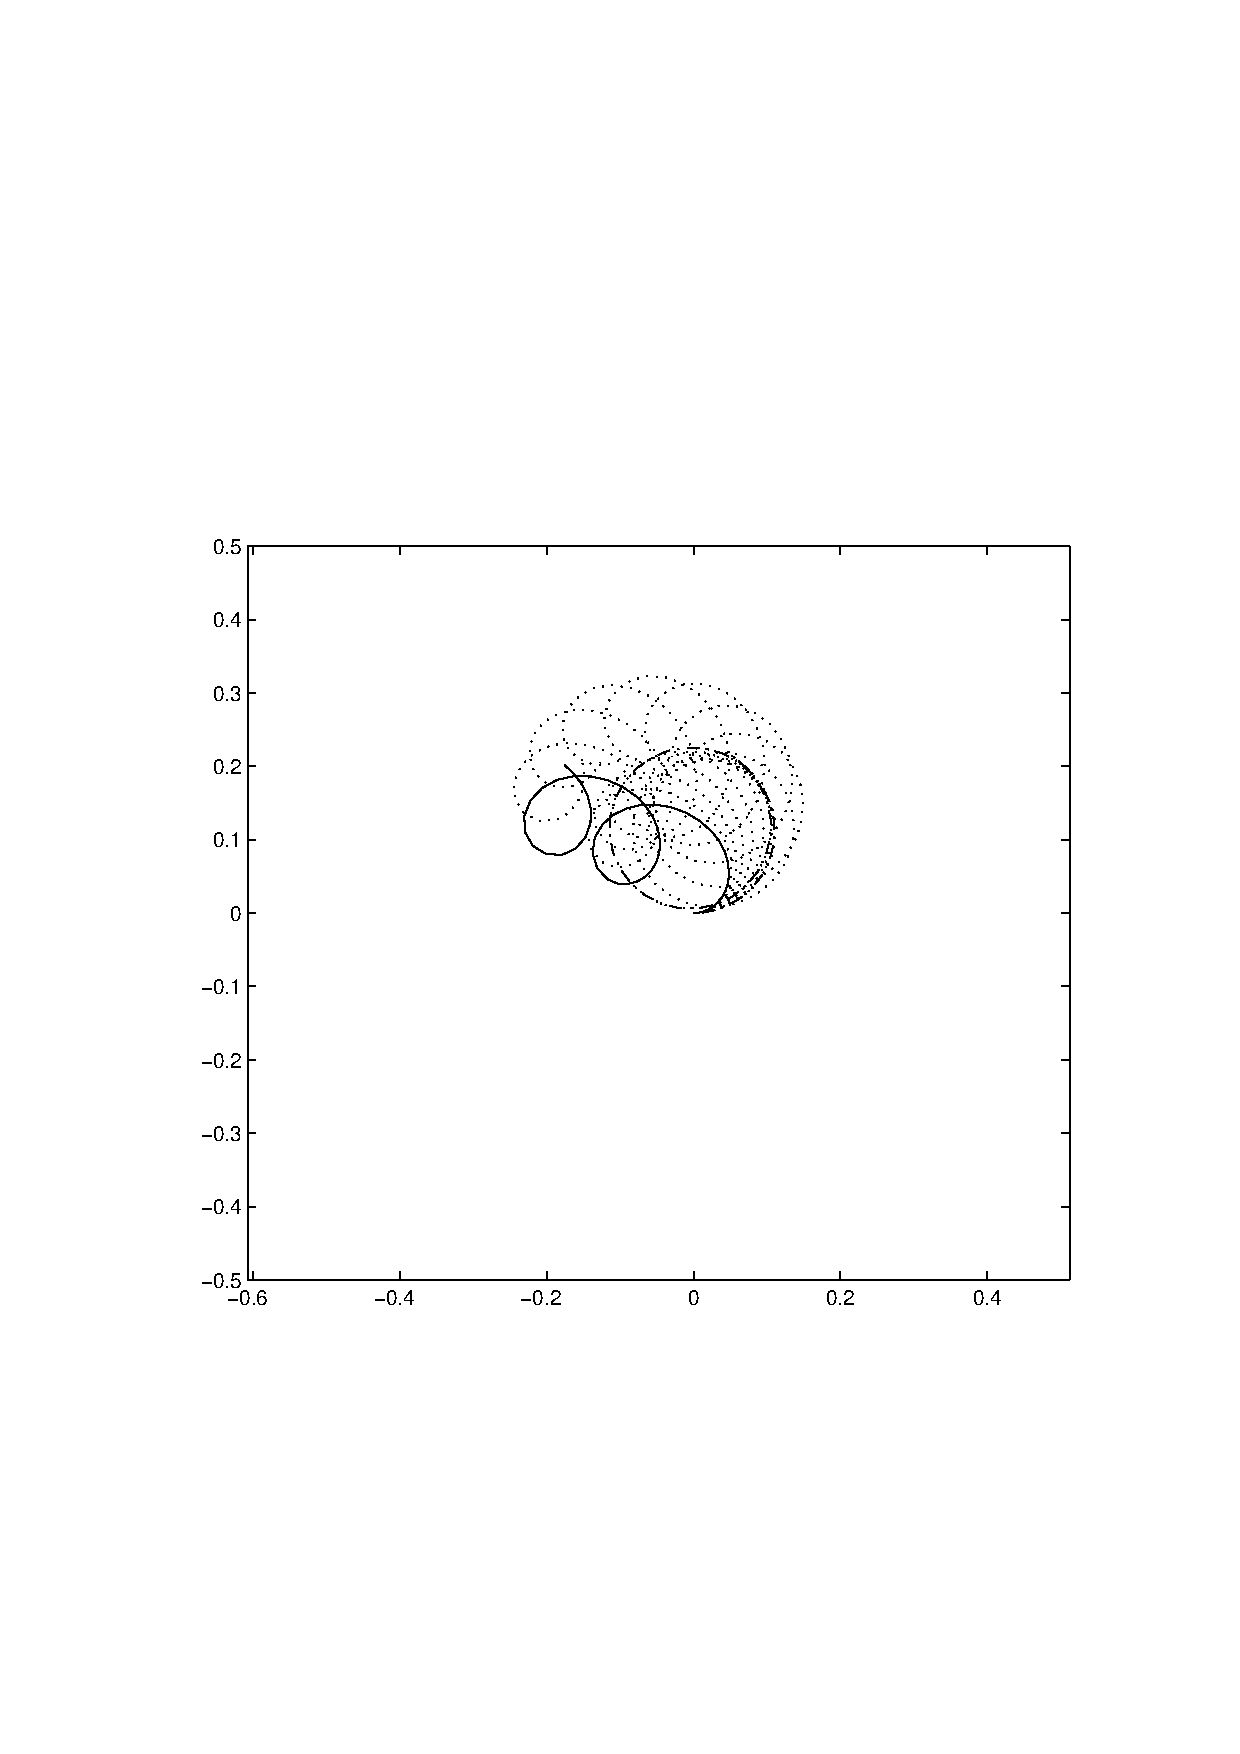
\includegraphics[height=6cm,width=6cm]{dataset2}
\caption{elastic data set 2}
\label{dataset2}
\end{center}
\end{figure} 


